%% 2019 NeuroFedora contributors

%% packages %%
% support for coloured text
\usepackage{xcolor}
\definecolor{FedoraBlue}{cmyk}{1.0,0.46,0.0,0.0}
\definecolor{FedoraDarkBlue}{cmyk}{1.0,0.57,0.0,0.38}
\definecolor{FriendsMagenta}{cmyk}{0.0,0.8,0.4,0.0}
\definecolor{FeaturesOrange}{cmyk}{0.0,0.5,1.0,0.0}
\definecolor{FirstGreen}{cmyk}{0.5,0.0,1.0,0.0}
\definecolor{FreedomPurple}{cmyk}{0.57,0.46,0.0,0.0}

% IPA
\usepackage{tipa}
\usepackage[scale=2]{ccicons}
\usepackage{amssymb}
\usepackage{tikz}
\usetikzlibrary{arrows.meta, arrows, positioning}
\usepackage{jneurosci}
\usepackage{subfig}
\usepackage[T1]{fontenc}
\usepackage[utf8]{inputenc}
\usepackage[style=verbose,backend=biber,autocite=footnote]{biblatex}
\addbibresource{masterbib.bib}
% Use opensans
\usepackage[default,osfigures,scale=0.95]{opensans}
% for strike through
\usepackage[normalem]{ulem}
% links, urls, refs
\usepackage{hyperref}
\hypersetup{colorlinks,linkcolor=FreedomPurple,urlcolor=FreedomPurple}
% graphics
\usepackage{graphicx}
% algorithm
\usepackage{algorithmic}
\usepackage{textcomp}
\usepackage{wrapfig}
\usepackage{textgreek}
\usepackage{euler}
% \usepackage{minted}

% beamer theme
\usetheme[numbering=fraction]{metropolis}
\usefonttheme[onlymath]{serif}
\setbeamerfont{footnote}{size=\tiny}
\setbeamerfont{caption}{size=\tiny}
\setbeamercolor{alerted text}{fg=FeaturesOrange}
\setbeamercolor{progress bar}{fg=FriendsMagenta}
\setbeamercolor{title separator}{fg=FriendsMagenta}
\setbeamercolor{frametitle}{bg=FedoraDarkBlue}

\renewcommand{\figurename}{}

% Not needed in metropolis, but in general footnote citation fixes: https://tex.stackexchange.com/questions/44217/how-can-i-stop-footcite-from-hijacking-my-beamer-columns
% how to use multiple references to the same footnote: https://tex.stackexchange.com/questions/27763/beamer-multiple-references-to-the-same-footnote

%% title %%
\title[NeuroFedora]{\includegraphics[keepaspectratio,width=.25\textwidth]{images/NeuroFedoraLogo01.png}\\NeuroFedora}
\subtitle{Free Software for Free Neuroscience}
\author{Ankur Sinha\\Ph.D. candidate: UH Biocomputation Group, UK,\\Volunteer: Fedora Project.}
\date[]{}
%% document begins %%
\begin{document}

% title frame %%
\begin{frame}
  \titlepage{}
\end{frame}

%% Three slides for 5 minutes, so 9 slides for 15 minutes.
\section{Free/Open (neuro) Science}
\begin{frame}[c]{Modern Free/Open Science}
  \note[item]{We know this, but it's always to remind ourselves how massive modern Open Science is.}
  \note[item]{It encompasses everything from data collection, to storage, to sharing, to processing, to dissemination of results.}
  \begin{figure}[htpb]
    \centering
    \includegraphics[width=\linewidth]{images/openscience-taxonomy.png}
  \end{figure}
  \footnotetext[1]{\href{https://en.wikipedia.org/wiki/Open\_science}{Petr Knoth and Nancy Pontika (CC BY 3.0)}}
\end{frame}
\begin{frame}[c]{The ideal, in short:}
  Free/Open Science:\\\alert{Everyone} should have the freedom to \alert{share, study, and modify} scientific material.\\
  \pause{}
  \vspace{0.5cm}
  \alert{Free/Open Science includes and relies heavily on Free/Open Source Software (FOSS).}\\
  \pause{}
  \vspace{0.5cm}
  FOSS\@:\\\alert{Everyone} should have the freedom to \alert{share, study, and modify} software\footnotemark[5].\\
  \footnotetext[2]{\href{https://u.fsf.org/user-liberation}{Free software foundation}}
\end{frame}
\begin{frame}[c]{So we strive to use more and more FOSS}
  \begin{figure}[htpb]
    \centering
    \includegraphics[width=\linewidth]{images/open-source-paper.png}
  \end{figure}
  \footnotetext[6]{\href{http://opensourceforneuroscience.org/}{Open source for neuroscience}}
\end{frame}
\section{NeuroFedora: why, how, what?}
\begin{frame}[c]{FOSS:\ Developers and users}
  \begin{figure}[h]
  \begin{center}
  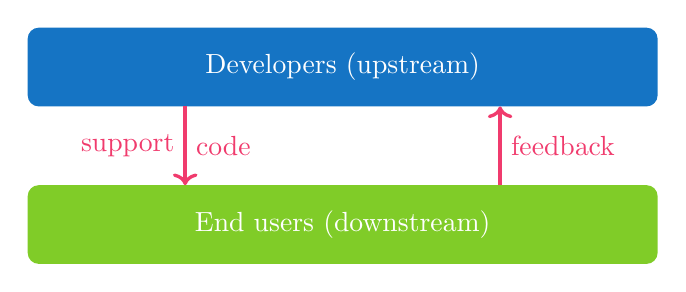
\begin{tikzpicture}[scale=1, transform shape]
    \fill[fill=FedoraBlue, text=white, rounded corners] (0, 0) rectangle ++(8, 1) node[pos=0.5] (A){Developers (upstream)};
    \fill[fill=FirstGreen, text=white, rounded corners] (0, -2) rectangle ++(8, 1) node[pos=0.5] (B){End users (downstream)};
    \draw [FriendsMagenta, very thick, ->] (2, 0) -- node [midway, right, text centered] {code} node [midway, left, text centered] {support} ++(0, -1) ;
    \draw [FriendsMagenta, very thick, ->] (6, -1) -- node [midway, right, text centered] {feedback} ++(0, 1);
  \end{tikzpicture}
  \end{center}
  \end{figure}
\end{frame}
\begin{frame}[c]{Neuroscience community: highly multidisciplinary}
  \begin{itemize}
    \item \alert{various specialities:} biologists, mathematicians, physicists, chemists, psychologists, \ldots, 
      \pause{}
    \item \alert{small proportion of trained software developers}
  \end{itemize}
\end{frame}
\begin{frame}[c]{(Anecdotal) notes on development of research software}
  \begin{itemize}
    \item often \alert{single developer}, or small development teams
    \item limited \alert{maintenance, short-lived projects}
    \item limited \alert{access to hardware/resources}
    \item limited \alert{code quality}
    \item limited \alert{use of established best practices}
    \item limited \alert{testing for correctness (!)}
    \item \alert{complex dependency chains}
    \item lack of \alert{documentation and support}
    \item lack of \alert{community development know-how}
  \end{itemize}
  \note[item]{Give how interdisciplinary neuroscience is, most researchers are NOT trained in development}
  \note[item]{This implies, and this is based on anecdotal evidence, that the software used in research is not of the best quality}
\end{frame}
\begin{frame}[c]{(Anecdotal) notes on users of research software}
  \begin{itemize}
    \item \alert{waste time and effort} installing (and reinstalling) their software stacks
    \item \alert{rarely run test suites (!)}
    \item \alert{rarely report bugs} upstream
    \item \alert{rarely send improvements} upstream
    \item are \alert{unaware of helpful development tools}
  \end{itemize}
  \note[item]{The other side of the bridge is the users}
  \note[item]{Because they aren't trained, they have a hard time setting up and using the software}
  \note[item]{If correctness of a tool cannot be verified, how can the correctness of the scientific result be claimed?}
\end{frame}
\begin{frame}[c]{Distributions liaison between developers and users}
  \begin{figure}[h]
  \begin{center}
  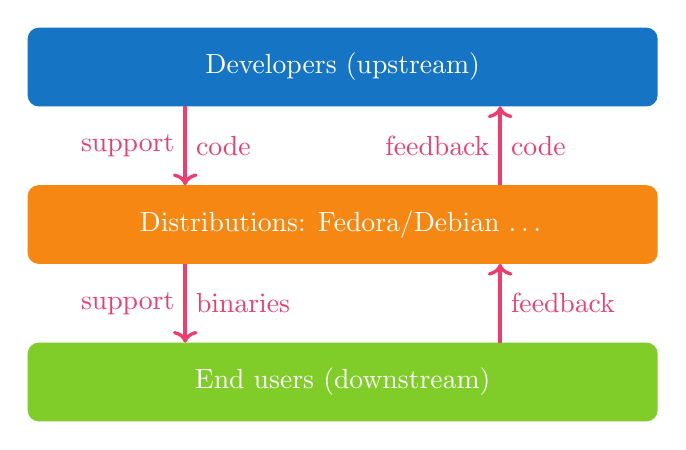
\begin{tikzpicture}[scale=1, transform shape]
    \fill[fill=FedoraBlue, text=white, rounded corners] (0, 0) rectangle ++(8, 1) node[pos=0.5] (A){Developers (upstream)};
    \fill[fill=FeaturesOrange, text=white, rounded corners] (0, -2) rectangle ++(8, 1) node[pos=0.5] (B){Distributions: Fedora/Debian \ldots};
    \draw [FriendsMagenta, very thick, ->] (2, 0) -- node [midway, right, text centered] {code} node [midway, left, text centered] {support} ++(0, -1) ;
    \draw [FriendsMagenta, very thick, ->] (6, -1) -- node [midway, right, text centered] {code} node [midway, left, text centered] {feedback} ++(0, 1) ;
    \fill[fill=FirstGreen, text=white, rounded corners] (0, -4) rectangle ++(8, 1) node[pos=0.5] (B){End users (downstream)};
    \draw [FriendsMagenta, very thick, ->] (2, -2) -- node [midway, right, text centered] {binaries} node [midway, left, text centered] {support} ++(0, -1) ;
    \draw [FriendsMagenta, very thick, ->] (6, -3) -- node [midway, right, text centered] {feedback} ++(0, 1) ;
  \end{tikzpicture}
  \end{center}
  \end{figure}
\end{frame}
\begin{frame}[c]{Distributions, like Fedora, are in a unique position:}
  \begin{itemize}
    \item \alert{liaison between upstream and users}
    \item have the \alert{infrastructure}
    \item \alert{follow best practices} in software development
    \item constantly \alert{work community development}
    \item \alert{learn from one another}---train while working
    \item \alert{disseminate} information to end-users
  \end{itemize}
\end{frame}
\begin{frame}[c]{NeuroFedora:}
  \textcolor{FedoraBlue}{Primary goal:}
  \begin{itemize}
    \item Provide a \alert{ready to use, integrated FOSS platform} for neuroscientists\footnotemark[7].
  \end{itemize}
  \pause{}
  \textcolor{FirstGreen}{Secondary/collateral goals:}
  \pause{}
  \begin{itemize}
    \item help \alert{improve the standard and maintenance} of tools
    \item help users \alert{develop software development skills}
    \item \alert{make neuroscience accessible} to non-specialists
  \end{itemize}
  \footnotetext[7]{Researchers, academics, hobbyists, anyone!}
\end{frame}
\begin{frame}[c]{NeuroFedora: current metrics}
  \begin{itemize}
    \item \alert{less than a year old\footnotemark[8],}
      \pause{}
    \item \textcolor{FirstGreen}{20 active contributors:}
      \begin{itemize}
        \item 15 package maintainers
        \item 5 designers, newcomers
        \item only 5 from a neuroscience background
      \end{itemize}
      \pause{}
    \item \textcolor{FriendsMagenta}{software:}
      \begin{itemize}
        \item 120 tools (packages) ready to install\footnotemark[9].
        \item \textasciitilde{}170 in queue\footnotemark[10].
      \end{itemize}
  \end{itemize}
  \footnotetext[8]{in its second iteration}
  \footnotetext[9]{\href{https://src.fedoraproject.org/group/neuro-sig}{src.fedoraproject.org: Neuro-SIG}}
  \footnotetext[10]{\href{https://pagure.io/neuro-sig/NeuroFedora/issues?status=Open&tags=T\%3A+Software}{Pagure.io: Neuro-SIG: issues}}
\end{frame}
\begin{frame}[c]{NeuroFedora is at:}
  \begin{columns}
   \begin{column}{0.3\textwidth}
      \begin{figure}[h]
        \centering
        \includegraphics[width=\linewidth]{images/NeuroFedoraBadge.png}
      \end{figure}
    \end{column}
    \begin{column}{0.8\textwidth}
      \textcolor{FedoraBlue}{Mailing list:\ neuro-sig@lists.fedoraproject.org}\\
      \textcolor{FirstGreen}{IRC:\ \#fedora-neuro on Freenode}\\
      \textcolor{FeaturesOrange}{Telegram:\ t.me/NeuroFedora}\\
      \textcolor{FriendsMagenta}{Documentation\ neuro.fedoraproject.org}\\
      \textcolor{FirstGreen}{Blog:\ neuroblog.fedoraproject.org}\\
      \textcolor{FeaturesOrange}{Pagure.io (FOSS Git forge):\ neuro-sig/NeuroFedora}
    \end{column}
  \end{columns}
\end{frame}
\end{document}
